% gc-05-TrigDiff.tex

\documentclass[xcolor=dvipsnames]{beamer}
\usepackage{teachbeamer}

\title{Differentiating Trigonometric Functions}
\subtitle{{\CourseNumber}, BCIT}

\author{\CourseName}

\date{January 22, 2018}

% \begin{figure}[h]
% 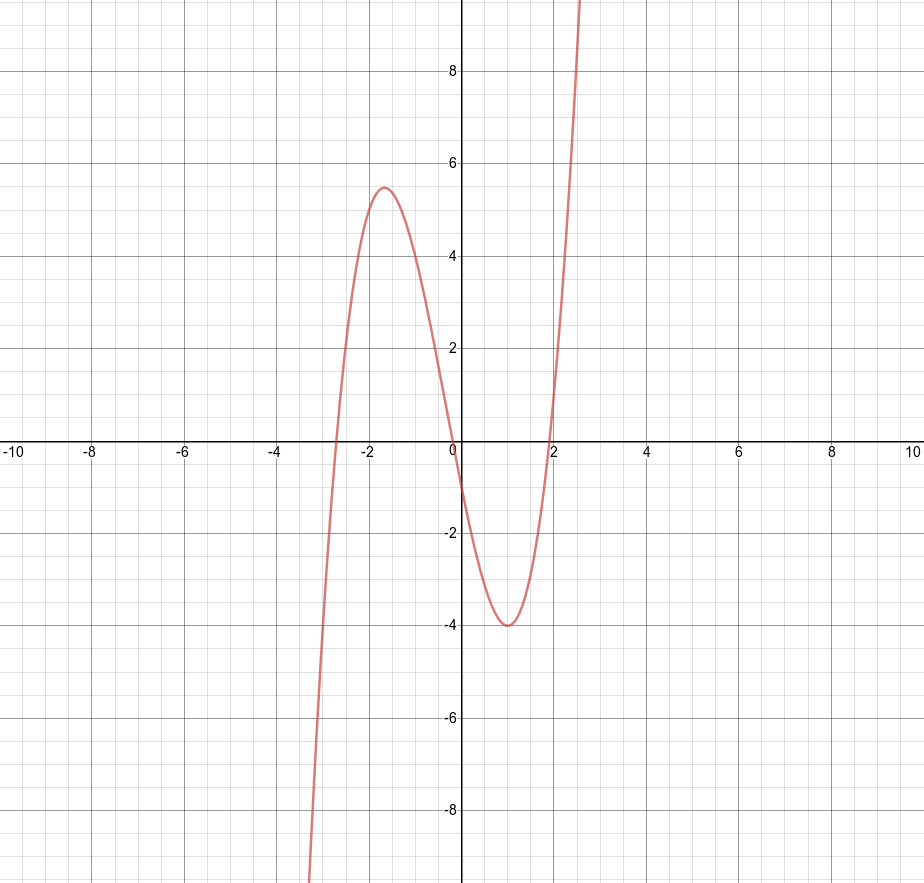
\includegraphics[scale=.3]{./diagrams/extrema1.png}
% \end{figure}

\begin{document}

\begin{frame}
  \titlepage
\end{frame}

\begin{frame}
  \frametitle{Trigonometric Functions Review}
Make sure to remember that the trigonometric functions (sine, cosine,
tangent, cotangent, etc.) are functions from the real numbers into the
real numbers. An angle is a real number in terms of its
\alert{radian} measure. If the angle is in degrees, it can be
converted to radians as in the following example,
\begin{equation}
  \label{eq:eedeehuc}
  42^{\circ}=42\cdot\frac{\pi}{180}\approx{}0.73304
\end{equation}
\end{frame}

\begin{frame}
  \frametitle{Trigonometric Functions Review}
  Any right triangle whose hypotenuse is of length $c'=1$ can be
  inserted into the unit circle so that one of the two shorter sides
  rests on the $x$-axis and one of the vertices is at the origin
  (reference triangle). Then the vertex $B$ in the diagram has the
  coordinates $(\cos\alpha,\sin\alpha)$.
    \begin{figure}[h]
    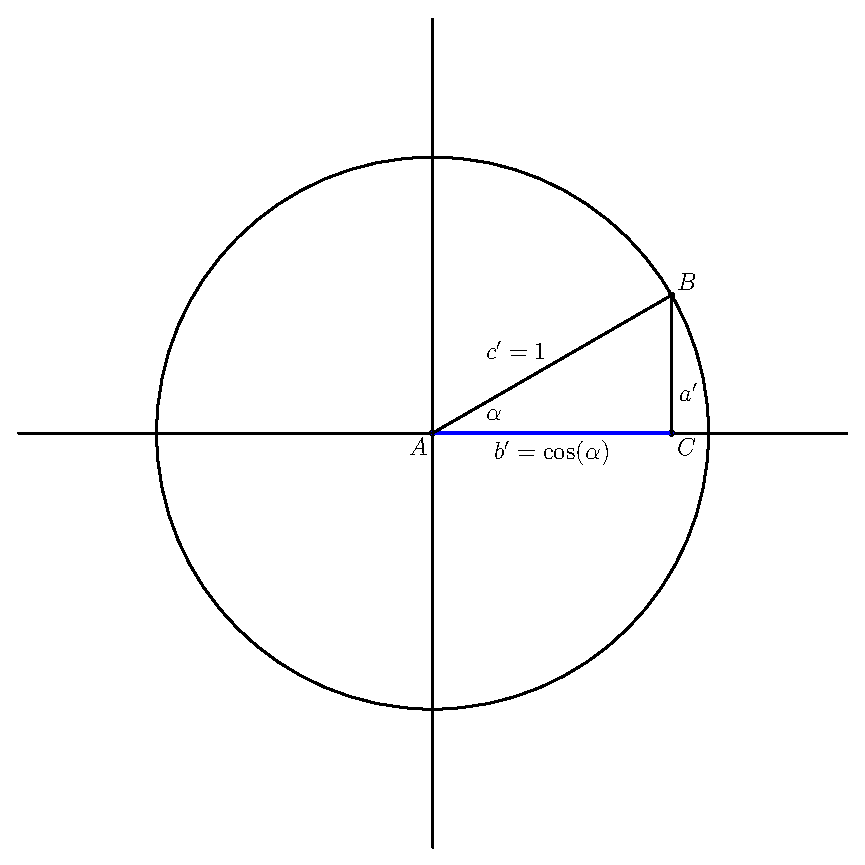
\includegraphics[scale=.45]{./diagrams/cosine.eps}
  \end{figure}
\end{frame}

\begin{frame}
  \frametitle{Trigonometric Functions Review}
  The remaining trigonometric functions are defined as follows.
  \begin{equation}
    \label{eq:eiyiexir}
    \tan{}x=\frac{\sin{}x}{\cos{}x}
  \end{equation}
  \begin{equation}
    \label{eq:dohquohb}
    \cot{}x=\frac{\cos{}x}{\sin{}x}=\frac{1}{\tan{}x}
  \end{equation}
  \begin{equation}
    \label{eq:eengohqu}
    \csc{}x=\frac{1}{\sin{}x}
  \end{equation}
  \begin{equation}
    \label{eq:eipuoxei}
    \sec{}x=\frac{1}{\cos{}x}
  \end{equation}
\end{frame}

\begin{frame}
  \frametitle{Trigonometric Functions Review}
  Here is a graph of the sine and cosine functions.
  \begin{figure}[h]
    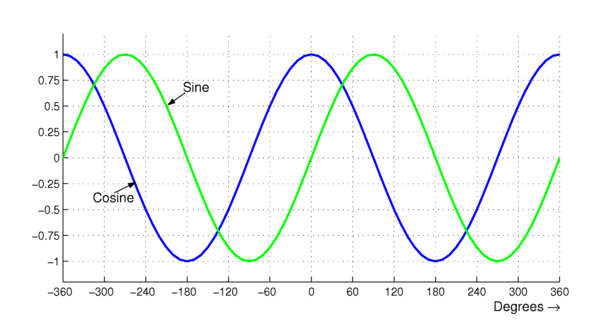
\includegraphics[scale=2]{./diagrams/sinecosine.png}
  \end{figure}
\end{frame}

\begin{frame}
  \frametitle{Trigonometric Functions Review}
  Here is a graph of the tangent function.
  \begin{figure}[h]
    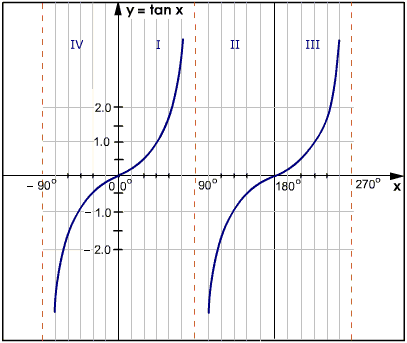
\includegraphics[scale=.5]{./diagrams/tangent.png}
  \end{figure}
\end{frame}

\begin{frame}
  \frametitle{Trigonometric Functions Review}
  Consider the following table of well-known inverse functions
  commonly used in calculus:

\bigskip

  \begin{tabular}{|l|l|}\hline
    \textbf{function} & \textbf{inverse} \\ \hline
    $e^{x}$ & $\ln{}x$ \\ \hline
    $\sin{}x$ & $\arcsin{}x\mbox{ or }\sin^{-1}$ \\ \hline
    $\cos{}x$ & $\arccos{}x\mbox{ or }\cos^{-1}$ \\ \hline
    $\tan{}x$ & $\arctan{}x\mbox{ or }\tan^{-1}$ \\ \hline
  \end{tabular}
\end{frame}

\begin{frame}
  \frametitle{Trigonometric Functions Review}
  Consider the following most important trigonometric identities:
  \begin{equation}
    \label{eq:shutooth}
    \sin^{2}x+\cos^{2}x=1
  \end{equation}
\begin{equation}
  \label{eq:iegaexah}
  \sin(-x)=-\sin{}x
\end{equation}
\begin{equation}
  \label{eq:gaijohra}
  \cos(-x)=\cos{}x
\end{equation}
\begin{equation}
  \label{eq:doajeigh}
  \tan(-x)=-\tan{}x
\end{equation}
\end{frame}

\begin{frame}
  \frametitle{Trigonometric Functions Review}
  Consider the following most important trigonometric identities:
\begin{equation}
  \label{eq:dieteipa}
  \sin(90^{\circ}-x)=\cos{}x
\end{equation}
\begin{equation}
  \label{eq:oepoodoh}
  \cos(90^{\circ}-x)=\sin{}x
\end{equation}
\begin{equation}
  \label{eq:aiwatong}
  \tan(90^{\circ}-x)=\cot{}x
\end{equation}
\begin{equation}
  \label{eq:jahpeexu}
  \sin(x+180^{\circ})=-\sin{}x
\end{equation}
\begin{equation}
  \label{eq:aephuemo}
  \cos(x+180^{\circ})=-\cos{}x
\end{equation}
\begin{equation}
  \label{eq:xaiyahcu}
  \tan(x+180^{\circ})=\tan{}x
\end{equation}
\begin{equation}
  \label{eq:aitahwae}
  \cot(x+180^{\circ})=\cot{}x
\end{equation}
\end{frame}

\begin{frame}
  \frametitle{Trigonometric Functions Review}
  Here are the angle sum identities,
  \begin{equation}
  \label{eq:eitaiquu}
  \sin(x+y)=\sin{}x\cos{}y+\cos{}x\sin{}y
\end{equation}
\begin{equation}
  \label{eq:iasoojou}
  \cos(x+y)=\cos{}x\cos{}y-\sin{}x\sin{}y
\end{equation}
from which we have, immediately following, the double angle
identities,
  \begin{equation}
    \label{eq:icuchodo}
    \sin(2x)=2\cos{}x\sin{}x
  \end{equation}
  \begin{equation}
    \label{eq:woojahtu}
    \cos(2x)=\cos^{2}x-\sin^{2}x
  \end{equation}
\end{frame}

\begin{frame}
  \frametitle{Limit of sin(x)/x}
\begin{figure}[h]
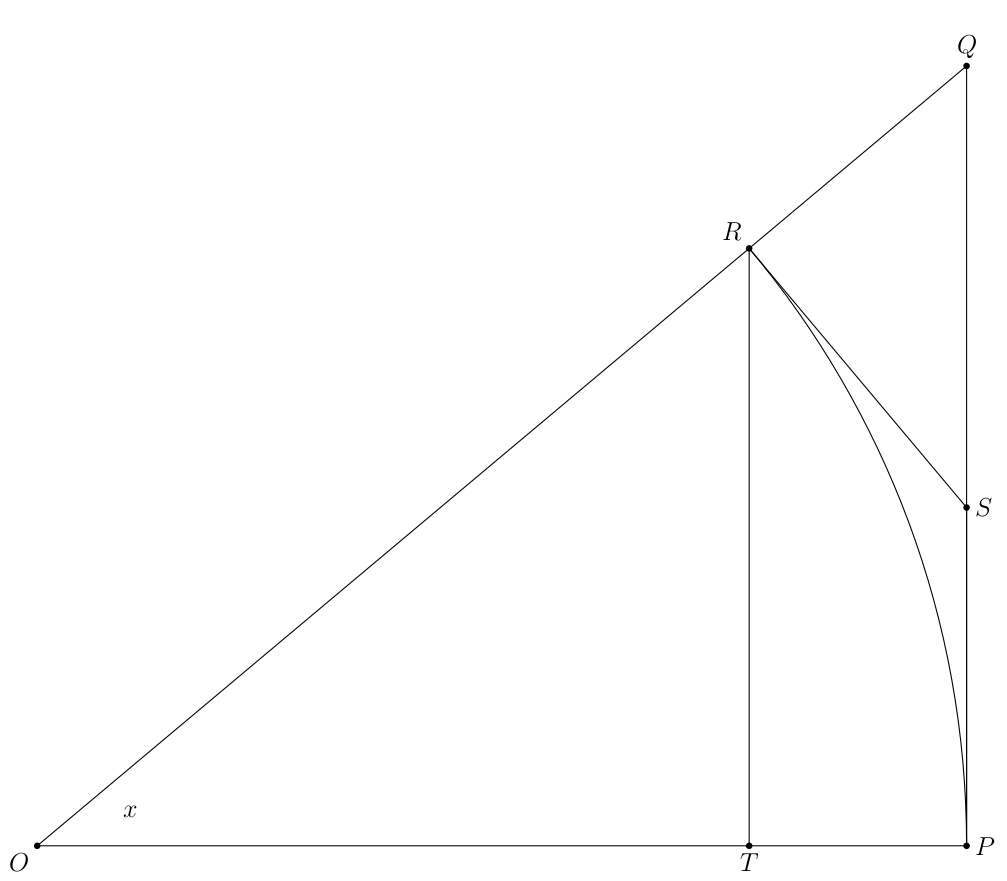
\includegraphics[scale=.24]{./diagrams/limsinxoverx.png}
\end{figure}
\end{frame}

\begin{frame}
  \frametitle{Limit of sin(x)/x}
  Let's find $\lim_{x\rightarrow{}0}\frac{\sin{}x}{x}$. On the last slide, consider the unit circle with
  $\|\vec{OP}\|=\|\vec{OR}\|=1$ and the angle $x$ at $O$. For simplicity let's
  assume that $0<x<\pi/2$. The angle $x$ is also the length of the arc
  between $P$ and $R$. Consequently
  \begin{equation}
    \label{eq:iufoobue}
\|\vec{RT}\|=\sin{}x\leq{}x    
  \end{equation}
  and therefore
  \begin{equation}
    \label{eq:chaveeju}
    \frac{\sin{}x}{x}\leq{}1
  \end{equation}
\end{frame}

\begin{frame}
  \frametitle{Limit of sin(x)/x}
  \begin{equation}
    \label{eq:uraewiha}
    x\leq\|\vec{PS}\|+\|\vec{SR}\|\leq\|\vec{PS}\|+\|\vec{SQ}\|=\|\vec{PQ}\|=\tan{}x
  \end{equation}
$\|\vec{SR}\|\leq\|\vec{SQ}\|$ because the angle $QRS$ is a right angle.
(\ref{eq:uraewiha}) means that
\begin{equation}
  \label{eq:uebaenih}
  \cos{}x\leq\frac{\sin{}x}{x}
\end{equation}
Since $\lim_{x\rightarrow{}0}\cos{}x=1$ and $\lim_{x\rightarrow{}0}1=1$, we can use the squeeze
theorem, (\ref{eq:chaveeju}), and (\ref{eq:uebaenih}) for
\begin{equation}
  \label{eq:guabighe}
  \lim_{x\rightarrow{}0}\frac{\sin{}x}{x}=1
\end{equation}
\end{frame}

\begin{frame}
  \frametitle{Limit of (cos(x)-1)/x}
  Consider
  \begin{equation}
    \label{eq:ungaeciz}
    \lim_{x\rightarrow{}0}\frac{\cos{}x-1}{x}=\lim_{x\rightarrow{}0}\left[\frac{\cos{}x-1}{x}\cdot\frac{\cos{}x+1}{\cos{}x+1}\right]=\notag
  \end{equation}
  \begin{equation}
    \label{eq:xiecahze}
    \lim_{x\rightarrow{}0}\frac{\cos^{2}x-1}{x(\cos{}x+1)}=-\lim_{x\rightarrow{}0}\left[\frac{\sin{}x}{x}\cdot\frac{\sin{}x}{\cos{}x+1}\right]=\notag
  \end{equation}
  \begin{equation}
    \label{eq:angoohee}
    -1\cdot\left(\frac{0}{1+1}\right)=0
  \end{equation}
\end{frame}

\begin{frame}
  \frametitle{Derivative of Sine}
  The derivative of $f(x)=\sin{}x$ is 
\begin{equation}
  \label{eq:eishooro}
  f'(x)=\lim_{h\rightarrow{}0}\frac{f(x+h)-f(x)}{h}=\lim_{h\rightarrow{}0}\frac{\sin(x+h)-\sin{}x}{h}=\notag
\end{equation}
\begin{equation}
  \label{eq:phauzelo}
  \lim_{h\rightarrow{}0}\frac{\sin{}x\cos{}h+\cos{}x\sin{}h-\sin{}x}{h}=\notag
\end{equation}
\begin{equation}
  \label{eq:jiexeedo}
  \lim_{h\rightarrow{}0}\left[\sin{}x\left(\frac{\cos{}h-1}{h}\right)+\cos{}x\left(\frac{\sin{}h}{h}\right)\right]=\cos{}x
\end{equation}
{\ubung} Differentiate $f(x)=x^{2}\sin{}x$.
\end{frame}

\begin{frame}
  \frametitle{The Derivative of Cosine}
The derivative of $f(x)=\cos{}x$ is 
\begin{equation}
  \label{eq:ahfiefev}
  f'(x)=-\sin{}x
\end{equation}
The proof is analogous to the proof for $\sin{}x$.

{\ubung} Differentiate 
\begin{equation}
  \label{eq:afeizeix}
  f(t)=\frac{1+\sin{}t}{t+\cos{}t}
\end{equation}
\end{frame}

\begin{frame}
  \frametitle{The Derivative of Tangent}
The derivative of $f(x)=\tan{}x$ is 
\begin{equation}
  \label{eq:uulohjeo}
  f'(x)=\sec^{2}x
\end{equation}
Use the quotient rule to prove this. Remember that 
\begin{equation}
  \label{eq:shooceid}
  \sec{}x=\frac{1}{\cos{}x}
\end{equation}
\end{frame}

\begin{frame}
  \frametitle{The Derivative of Arcsine}
  {\ubung} Find the following arcsine values:
  \begin{equation}
    \label{eq:ahquoila}
    \arcsin(-1)\hspace{.5in}\arcsin(1)\notag
  \end{equation}
  \begin{equation}
    \label{eq:eengaine}
    \arcsin\left(\frac{1}{2}\right)\hspace{.5in}\arcsin\left(\frac{\sqrt{3}}{2}\right)\hspace{.5in}\arcsin\left(-\frac{1}{\sqrt{2}}\right)\notag
  \end{equation}
  % \begin{tabular}{|l|l|}\hline
  %   $\arcsin(-1)$ & \\ \hline
  %   $\arcsin(1)$ & \\ \hline
  %   $\arcsin\left(\frac{1}{2}\right)$ & \\ \hline
  %   $\arcsin\left(\frac{\sqrt{3}}{2}\right)$ & \\ \hline
  %   $\arcsin\left(-\frac{1}{\sqrt{2}}\right)$ & \\ \hline
  % \end{tabular}
\begin{figure}[h]
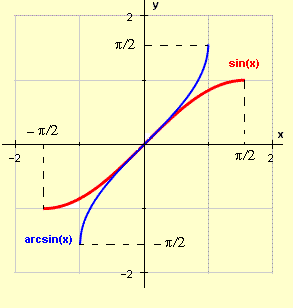
\includegraphics[scale=.5]{./diagrams/arcsin.png}
\end{figure}
\end{frame}

\begin{frame}
  \frametitle{The Derivative of Arcsine}
  We can tell from the graph that
  \begin{enumerate}
  \item $\frac{d}{dx}\arcsin{}x$ will be positive
  \item $\frac{d}{dx}\arcsin{}x$ will be defined on the interval $[-1,1]$
  \end{enumerate}
Let's restrict our attention to the first quadrant so that we may say
with confidence for $f(x)=\arcsin{}x$ that
\begin{equation}
  \label{eq:sieheuvu}
  sin(f(x))=x\mbox{ and therefore }\cos{}f(x)=\sqrt{1-\sin^{2}f(x)}
\end{equation}
\end{frame}

\begin{frame}
  \frametitle{The Derivative of Arcsine}
Take the equation $\sin(f(x))=x$ and differentiate with respect to $x$
on both sides.
\begin{equation}
  \label{eq:heipaeng}
  \sin(f(x))=x
\end{equation}
\begin{equation}
  \label{eq:xohtavie}
  \frac{d}{dx}\sin(f(x))=\frac{d}{dx}x
\end{equation}
We know the right-hand side equals 1. For the left-hand side, we that
\begin{equation}
  \label{eq:keeshoot}
  \frac{d}{dx}\sin{}x=\cos{}x
\end{equation}
but be very careful here
\begin{equation}
  \label{eq:ungitoov}
  \frac{d}{dx}\sin(f(x))\alert{\neq}\cos{}f(x)
\end{equation}
\end{frame}

\begin{frame}
  \frametitle{Derivatives of Trigonometric Functions}
\begin{figure}[h]
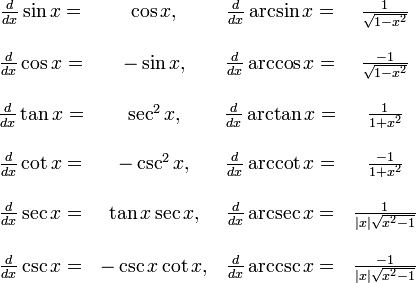
\includegraphics[scale=.6]{./diagrams/trigdiff.png}
\end{figure}
\end{frame}

\begin{frame}
  \frametitle{Exercises}
{\ubung} Differentiate the following function:
\begin{equation}
  \label{eq:hupuxahz}
  f(x)=3x^{2}-2\cos{}x
\end{equation}
{\ubung} Find the equation of the tangent line at $(\pi/3,2)$ for
\begin{equation}
  \label{eq:hoirohfo}
  y=\sec{}x
\end{equation}
\end{frame}

\begin{frame}
  \frametitle{Exercises}
{\ubung} Differentiate the following function:
\begin{equation}
  \label{eq:vithooke}
  f(x)=\sqrt{x}\sin{}x
\end{equation}
{\ubung} Find the equation of the tangent line at $(\pi/6,4+\frac{5}{2}\sqrt{3})$ for
\begin{equation}
  \label{eq:chaequin}
  f(x)=2\csc{}x+5\cos{}x
\end{equation}
\end{frame}

\begin{frame}
  \frametitle{Exercises}
{\ubung} Differentiate the following functions:
\begin{equation}
  \label{eq:hohxenoo}
  g(t)=4\sec{}t+\tan{}t
\end{equation}
\begin{equation}
  \label{eq:zichoope}
  f(x)=\csc{}x(x+\cot{}x)
\end{equation}
\begin{equation}
  \label{eq:tohsohgh}
  v(w)=\frac{\sin{}w}{w^{2}}
\end{equation}
\end{frame}

\begin{frame}
  \frametitle{End of Lesson}
Next Lesson: Chain Rule
\end{frame}

\end{document}
